\documentclass{article}
\usepackage[polish]{babel}
\usepackage[T1]{fontenc}
\usepackage[utf8]{inputenc}
\usepackage{polski}   
\usepackage{graphicx}   % rysunki
\usepackage{listings}   % kody programów

\def\TytulPolski    {Attendance Manager}
\def\NazwaSys {Attendance Manager}

\def\Student     {Jakub Piotr\\ Wojciech Agaciński\\ Krzysztof Adamczak}

%Kierunek:
\def\Kierunek {Informatyka}
 
%Specjalnosc:
\def\Specjalnosc {Technologie informatyczne}
% \def\Specjalnosc {Bezpieczeństwo systemów informatycznych} 

%Poziom studiów: 
\def\PoziomStudiow {I stopnia}
%\def\PoziomStudiow {II stopnia}

%Forma studiów:
\def\FormaStudiow {stacjonarne}
\AtBeginDocument{
    \renewcommand*{\tablename}{Tabela}
    \renewcommand*{\figurename}{Rys.} 
}

% Jeżeli kody programów zawierają polskie litery należy dodać odpowiedni znak poniżej
\lstset{literate=%
    {ż}{{\.z}}1
    {ą}{{\c{a}}}1
    {ę}{{\c{e}}}1
		{ó}{{\'o}}1
		{ć}{{\'c}}1
		{ś}{{\'s}}1
}
        



\title{\TytulPolski}
\author{\Student}

\begin{document}
% strona tytułowa: Politechnika Poznańska  Wydział Elektryczny  Instytut Automatyki i Inżynierii Informatycznej
% Imie Nazwisko
% Praca dyplomowa inżynierska
% Tutuł pracyy 
% promotor: dr inż. Imię Nazwisko
% Poznań, 2017
% \maketitle
\thispagestyle{empty}
\begin{center}
Politechnika Poznańska\\
Wydział Elektryczny\\  
Instytut Automatyki i Inżynierii Informatycznej\\
 % \vspace{5mm}
\begin{figure}[ht!]
%\centering
\hspace{47mm}\includegraphics[width=50mm,natwidth=421,natheight=421]{pplogo.png}
\end{figure}
  \vspace{5mm}
\large{\Student}\\
  \vspace{10mm}
\large{\TytulPolski}\\
  \vspace{10mm}
\end{center}
\vspace{50mm}

\vspace{10mm}
\begin{center}
Poznań, 2017
\end{center}
 
        % strona tytułowa
\newpage\tableofcontents     % Spis tresci
\newpage\section{Wstęp}\label{sec:wstep}
\subsection{Cel i zakres pracy}
% Odpowiedź na pytanie: Do czego system służy?
% Przedstawić zadania szczegółowe z karty tematu 

System ma za zadanie monitorować obecności studentów na zajęciach laboratoryjnych, wykorzystując istniejącą infrastrukturę informatyczną, tj. czytniki kart inteligentnych zainstalowane w komputerach oraz legitymacje studenckie.
% Priorytet: Wysoki, Średni, Niski
\begin{table}[!ht]
\centering
    \begin{tabular}{|c|p{6cm}|c|c|}
        \hline
        \textit{Lp.} & \textit{Opis funkcjonalności} & \textit{Dostępność}  & \textit{Priorytet} \\ \hline
        1. & Odczytanie danych z legitymacji & - & Wysoki \\ \hline
        2. & Ręczne wprowadzenie danych o obecności& a & Średni \\ \hline
        3. & Dostęp do panelu administracyjnego prez web serwis & a & Wysoki \\ \hline
        4. & Podgląd istniejących w systemie wydarzeń & a & Wysoki \\ \hline
        5. & Planowanie wydarzeń jednorazowych & a & Wysoki \\ \hline
        6. & Planowanie wydarzeń cyklicznych & a & Wysoki \\ \hline
        7. & Ustalanie list dopuszczonych do wydarzenia uczestnikow & a & Średni \\ \hline
    \end{tabular}
    \caption{Funkcjonalność systemu \NazwaSys (a -- administrator)}
    \label{table:tab1}
\end{table}

\subsection{Podział pracy}

\begin{table}[h!]
\centering
    \begin{tabular}{|p{4cm}|p{5cm}|}
        \hline
        \textit{Osoba odpowiedzialna} & \textit{Zadanie} \\ \hline
        Krzysztof Adamczak & Front end, Web serwis \\ \hline
        Wojciech Agaciński & Web serwis, Baza danych  \\ \hline
        Jakub Piotr & Aplikacja kliencka  \\  \hline
    \end{tabular} 
    \caption{Podział pracy}
    \label{table:tab2}
\end{table}          % wstep
% 
\newpage\section{Opis dziedziny przedmiotowej pracy}\label{sec:dziedzina}
\subsection{Pojęcia i definicje}
\subsection{Stan wiedzy}
\subsection{Dyskusja} 
      % wprowadznie do tematu pracy 
\newpage\section{Wybór technologii informatycznych} \label{sec:technologie}
\subsection{ASP.NET MVC}
Informacje o asp.net mvc i argumenty {Wojtek}
\subsection{Front End}
\subsection{.NET applikacja}
\subsection{Latex do dokumentacji}
\subsection{Format JSON}
(ang. \textit{JavaScript Object Notation}) \cite{json2017}
\subsection{Środowisko programistyczne Visual Studio}    % opis technologii informatycznych wykorzystanych w pracy
% Dokumentacja projektowa 
\newpage\section{Architektura systemu \NazwaSys}\label{sec:model}
% Odpowiedź na pytanie: Jak system działa?
\subsection{Schemat bazy danych} 
\begin{figure}[h!]
\centering
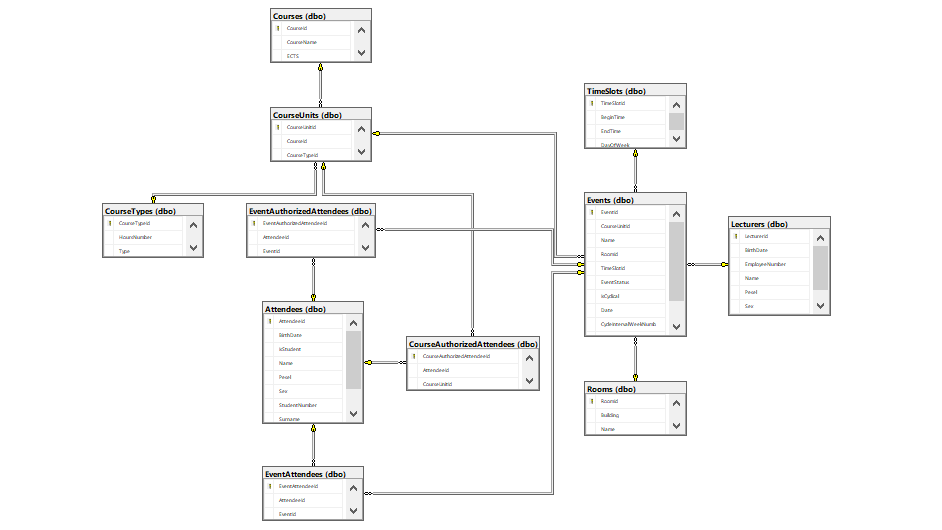
\includegraphics[width=16cm]{BD.png}
\caption{Schemat bazy danych}
\label{fig:schemat}
\end{figure}

\subsection{Moduł importu i eksportu danych}
Inferfejs administracyjny systemu podczas działania korzysta z interfejsu webowego stworzonego zgodnie z zasadami REST. Interfejs ten wykorzystuje notację JSON do serializacji zwracanych danych oraz protokół HTTP do komunikacji.

\subsection{Wnioski}
\begin{itemize}
    \item Wykorzystanie wzorca REST API oraz formatu danych JSON pozwala integrację systemu z innymi modułami stworzonymi na dowolnej platformie z wykorzystaniem dowolnego języka programowania wspierającego w.w. technologie.
\end{itemize}
          % dokumentacja projektowa
\newpage\section{Implementacja} \label{sec:implementacja}
\subsection{Wzorce projektowe i strukturalne}
\begin{itemize}  
    \item Model View Controller - wzorzec strukturalny wspierający zasadę Separation of Concerns - podział części serwerowej systemu na częsci odpowiedzialne za widoki, logikę biznesową oraz obsługę zapytań HTTP
    \item Inversion of Control - wzorzec strukturalny odpowiedzialny za zapewnienie luźnego powiązania pomiędzy klasami i likwidowanie zależności poprzez wykorzystanie Wstrzykiwania Zależności.
    \item Unit of Work - wzorzec projektowy zapewniający operowanie na jednej jednostce transakcji bazodanowych w obrębie zapytania do serwisu
    \item Repository Pattern - wzorzec projektowy zapewniający spójny format operacji CRUD na różnych strukturach danych 
\end{itemize}
\subsection{Model struktur danych}
Struktury danych odzwierciedlone w strukturach bazodanowych składają się z klas według modelu Plain Old CLR Object
\subsection{Model klas}
Podstawowe klasy występujące w systemie
\begin{itemize}
    \item Attendee - uczestnik wydarzenia
    \item Course - przedmiot dydaktyczny
    \item CourseType - rodzaj zajęć
    \item CourseUnit - jednostka dydaktyczna obejmująca przedmiot oraz rodzaj zajęć
    \item Event - wydarzenie
    \item Lecturer - wykładowca, prowadzący zajęcia
    \item Room - pomieszczenie
    \item TimeSlot - przedział czasowy
\end{itemize}
Podstawowe klasy występujące w aplikacji klienckiej.
\begin{itemize}
    \item ElectronicStudentCardData - model do przechowywania danych z ELS
    \item User - klasa która na podstawie klasy ElectronicStudentCardData tworzy użytkownika.
    \item CElectronicStudentCardContactDataReader - klasa zajmuje się odczytaniem danych z ELS
    \item ACR122UReader - klasa obsługująca czytnik ELS
    \item Event - wydarzenie
\end{itemize}




 
  % dokumentacja programistyczna
\newpage\section{Bezpieczeństwo systemu \NazwaSys} \label{sec:bezpieczenstwo}
\subsection{Anonimizacja danych}
W przypadku tworzenia raportow oraz danych statystycznych na podstawie informacji zebranych przez system dane powinny być anonimizowane, aby osoby postronne nie miały dostępu do wrażliwych danych
\subsection{Techniki kryptograficzne}
Techniki kryptograficzne mogą zostać wykorzystane do zabezpieczenia wrażliwych danych w systemie, m. in haseł użytkownika czy numerów PESEL uczestników wydarzeń.

 
 % analiza aspektów bezpieczeństwa systemu
\newpage\section{Instrukcja użytkowania aplikacji \NazwaSys} \label{sec:instrukcja}

\subsection{Strona główna}
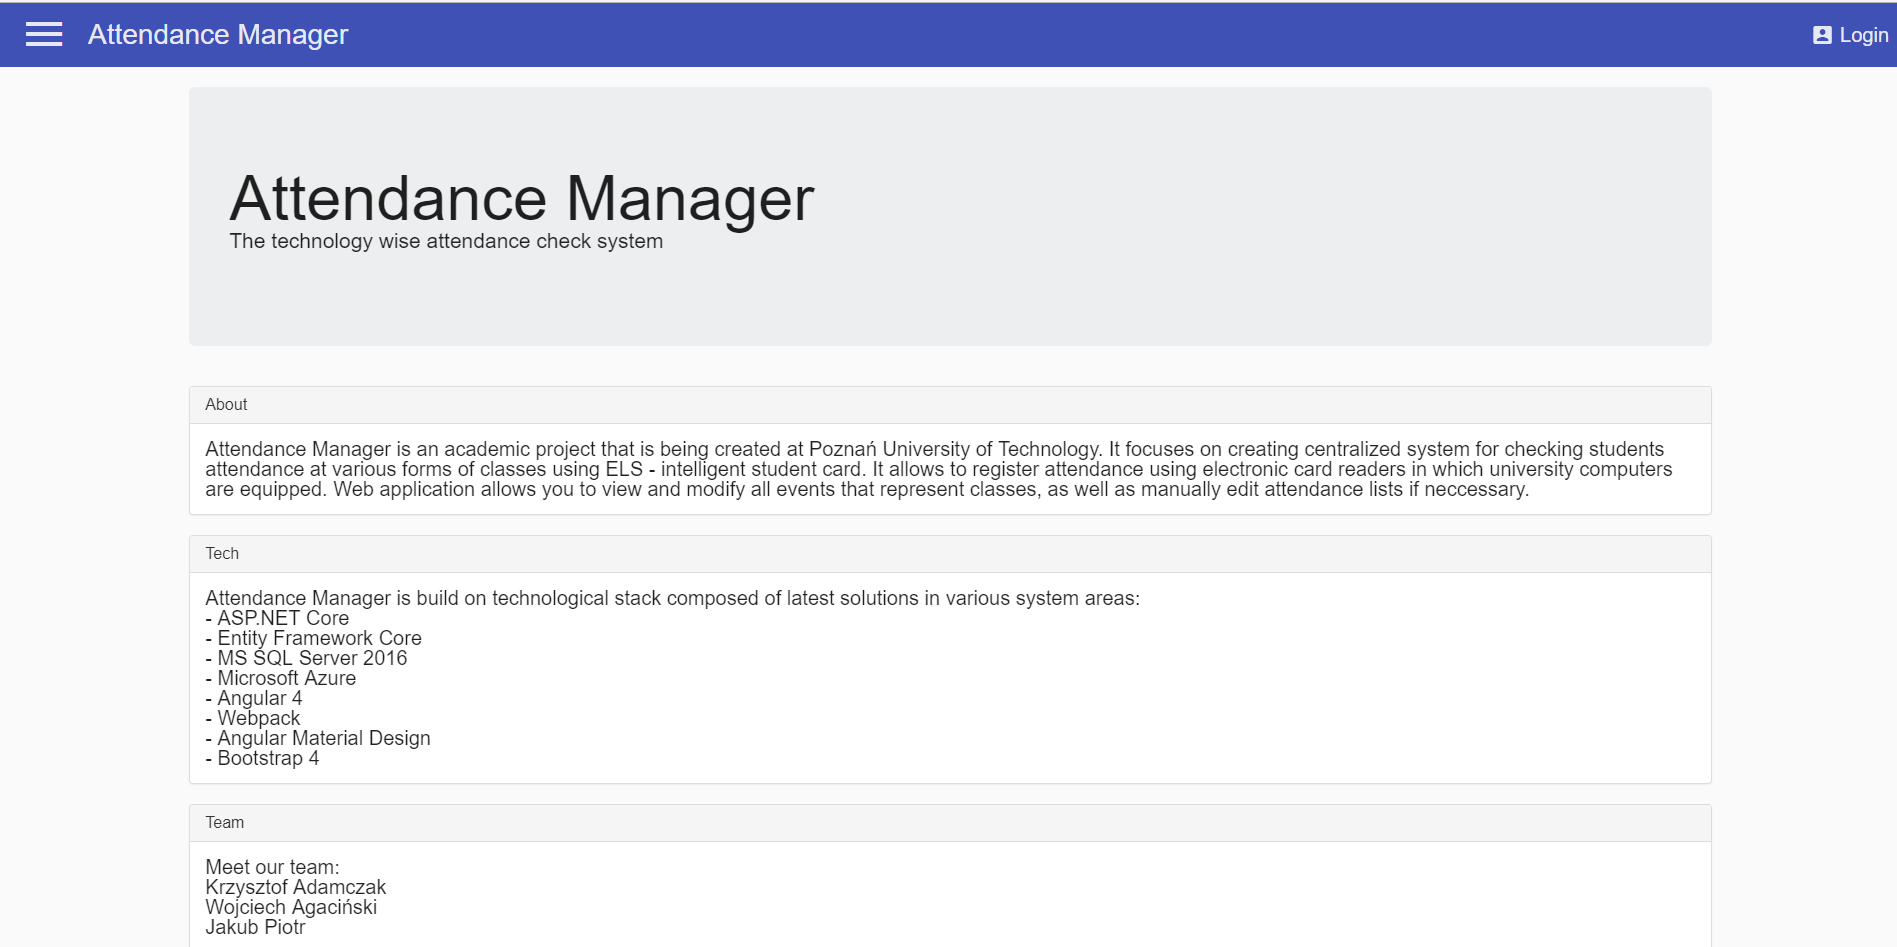
\includegraphics[height=8cm,width=15cm]{images/MainScreen}
Strona główna aplikacji zawiera podstawowe informacje dotyczące projektu takie jak: tytuł, opis, technologie oraz skład zespołu. W menu aplikacji po lewej stronie znajduje się przycisk otwierający menu główne aplikacji. W menu aplikacji mamy do wyboru następujące ekrany:
\begin{itemize}
    \item Home - prowadzi do strony startowej aplikacji (strony obecnej na zdjęciu)
    \item Events - strona z listą wydarzeń
    \item Add event - strona służąca do utworzenia nowego wydarzenia
\end{itemize}

\subsection{Lista wydarzeń - Active \& Incoming}
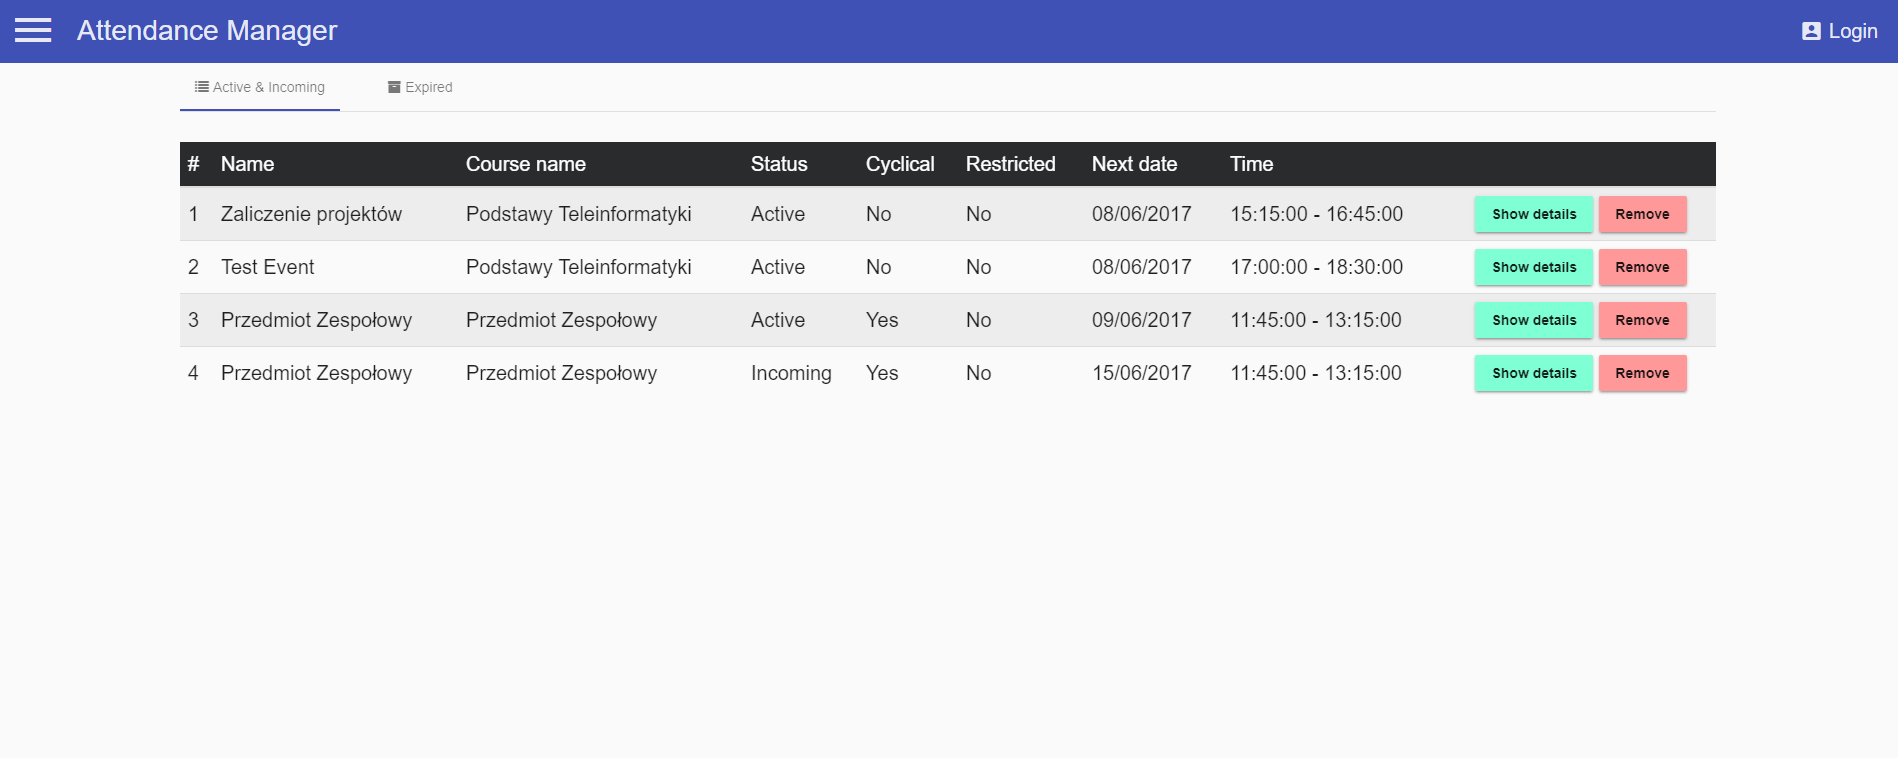
\includegraphics[height=8cm,width=15cm]{images/EventsListIncomingAndActive}
Jest to strona zawierająca listę wydarzeń. Została ona podzielona na dwie zakładki:
\begin{itemize}
    \item Active & Incoming - zakładka zawiera tabelę z wydarzeniami nadchodzącymi oraz aktywnymi
    \item Expired - zakładka zawiera tabelę z wydarzeniami które już się wydarzyły i zakończyły
\end{itemize}
Na powyższym zdjęciu przedstawiona została zakładka `Active & Incoming`. Zawiera ona tabelę wydarzeń nadchodzących oraz aktywnych. W tabeli znajdują się pola:
\begin{itemize}
    \item Name - kolumna zawierająca nazwę wydarzenia
    \item Course name - jest to nazwa kursu do którego przypisane zostało dane wydarzenie
    \item Status - jest to obecny status wydarzenia ('Active' lub 'Incoming')
    \item Cyclical - pola informujące czy wydarzenie jest jest cykliczne
    \item Restricted - pole informujące czy wydarzenie ma ograniczoną listę uczestników mogących wziąć udział w wydarzeniu
    \item Next date - kolumna z datą wydarzenia
    \item Time - kolumna z przedziałem czasowym w którym wystąpi wydarzenie
\end{itemize}
W ostatniej kolumnie znajdują się przyciski akcji.
\begin{itemize}
    \item Show details - po wciśnięciu tego przycisku nastąpi przeniesienie na stronę zawierająca wszystkie informacje na temat wybranego wydarzenia
    \item Remove - przycisk służący usunięcie wybranego wydarzenia
\end{itemize}

\subsection{Lista wydarzeń - Expired}
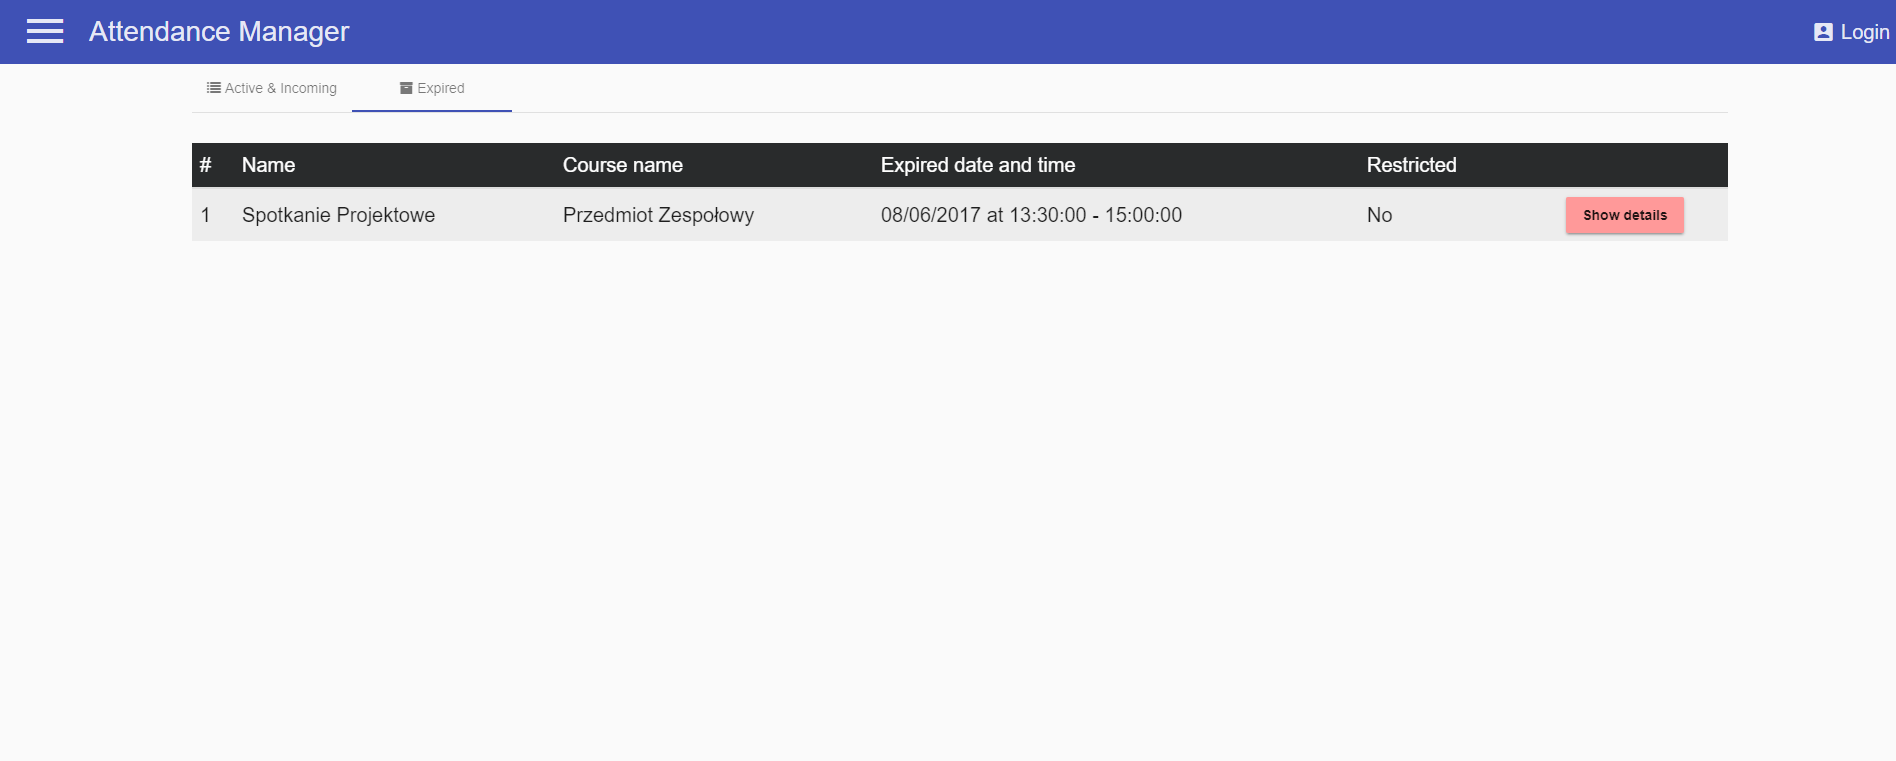
\includegraphics[height=8cm,width=15cm]{images/EventsListExpired}
Na powyższym zdjęciu przedstawiona została zakładka z wydarzeniami już zakończonymi. Zawiera ona tabelę z następującymi kolumnami:
\begin{itemize}
    \item Name - kolumna zawierająca nazwę wydarzenia
    \item Course name - jest to nazwa kursu do którego przypisane zostało dane wydarzenie
    \item Expired date and time - kolumna ta zawiera datę oraz przedział czasowy w którym odbyło się wydarzenie
    \item Restricted - pole informujące czy wydarzenie ma ograniczoną listę uczestników mogących wziąć udział w wydarzeniu
\end{itemize}
W tabeli znajduję się także przycisk 'Show details' który umożliwia podgląd szczegółów danego wydarzenia.

\subsection{Strona ze szczegółami wydarzenia}
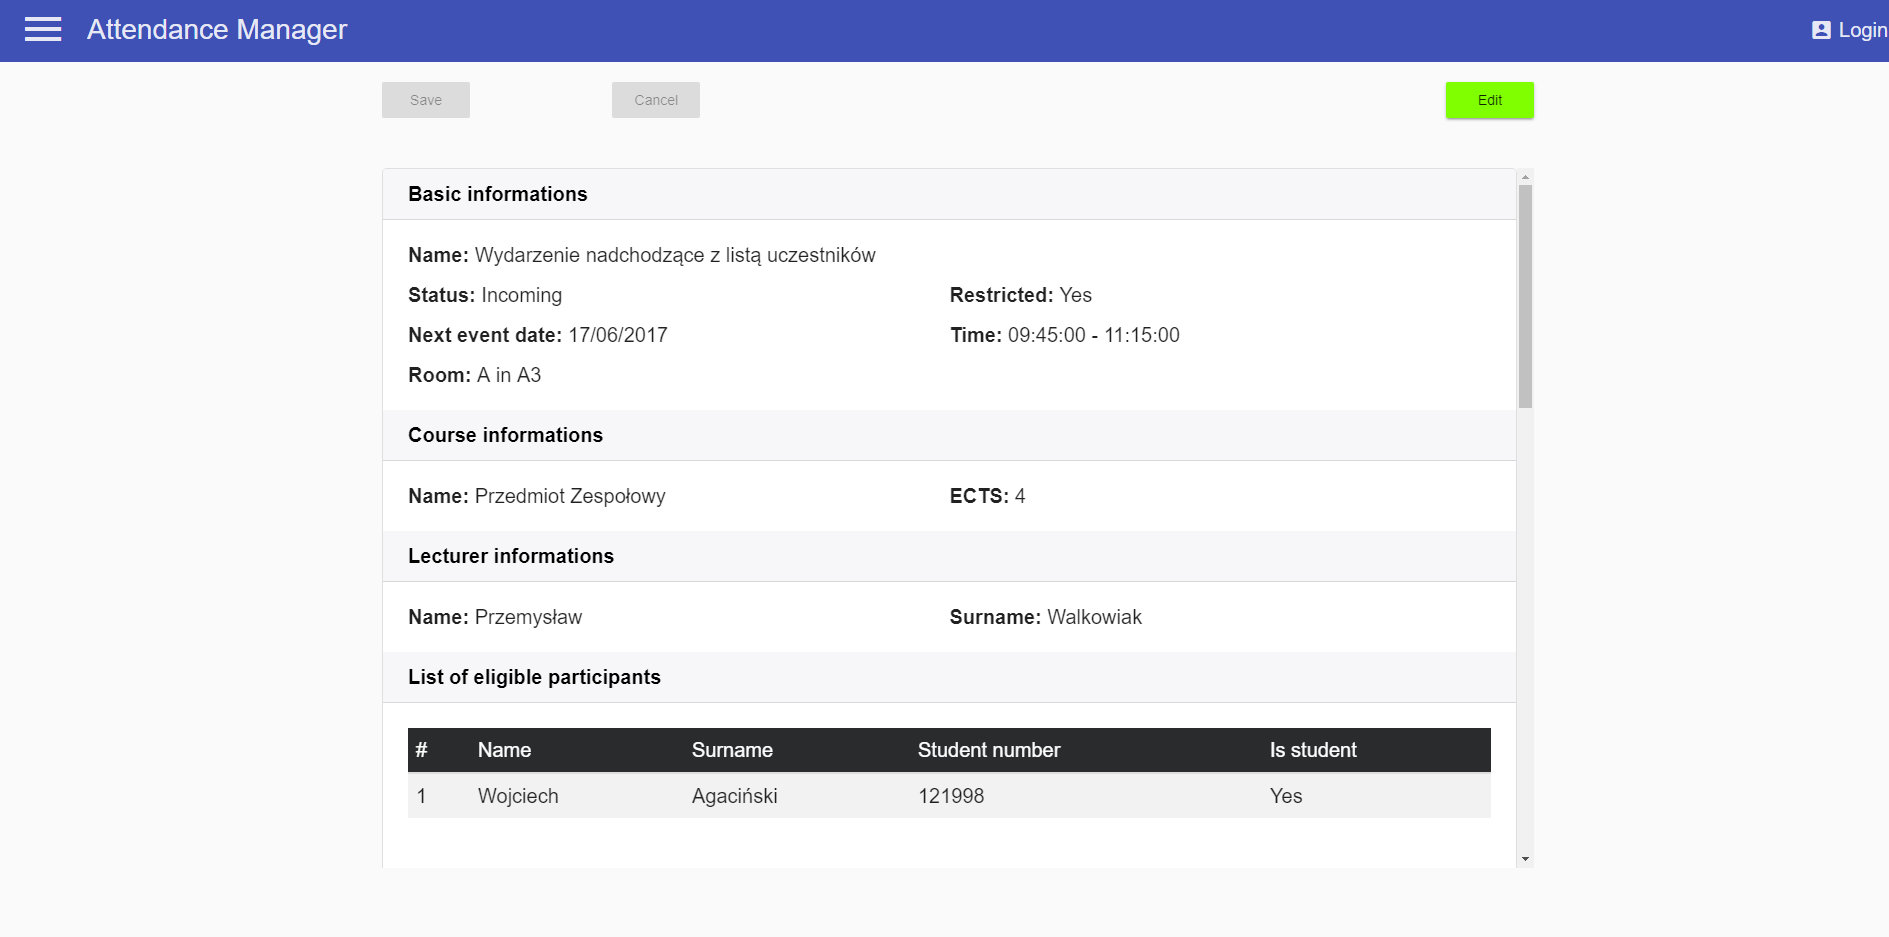
\includegraphics[height=8cm,width=15cm]{images/EventIncomingDetails}
Strona ta zawiera szczegółowe informacje na temat wydarzenia. Informacje zostały podzielone na sekcje:
\begin{itemize}
    \item Basic informations - sekcja zawierająca podstawowe informacje o wydarzeniu
    \item Course informations - sekcja zawierająca informację o kursie do którego podpięte jest wydarzenie. Sekcja ta jest opcjonalna. W przypadku braku podpietego kursu sekcja ta nie zostanie wyświetlona
    \item Lecturer informations - sekcja zawierająca informację o przypisanym do wydarzenia wykładowcy
    \item List of eligible participants - w przypadku gdy wydarzenie jest zamknięte (posiada listę uczestników uprawnionych do wzięcia udziału w wydarzeniu) pojawia się sekcja z listą uprawnionych uczestników
    \item Attendance list - sekcja zawierająca listę obecności. Pojawia się w przypadku gdy event jest aktywny lub zakończony
\end{itemize}
Na tej stronie możliwa jest edycja wydarzenia. W zależności od statusu wydarzenia niektóre pola/sekcje mogą być niedostępne do edytowania.
\begin{itemize}
    \item Wydarzenie nadchodzące - możliwa jest edycja prawie wszystkich pól oprócz listy obecności
    \item Wydarzenie aktywne - możliwa jest edycja jedynie listy obecności
    \item Wydarzenie zakończone - możliwa jest edycja jedynie listy obecności
\end{itemize}

\subsection{Tworzenie nowego wydarzenia}
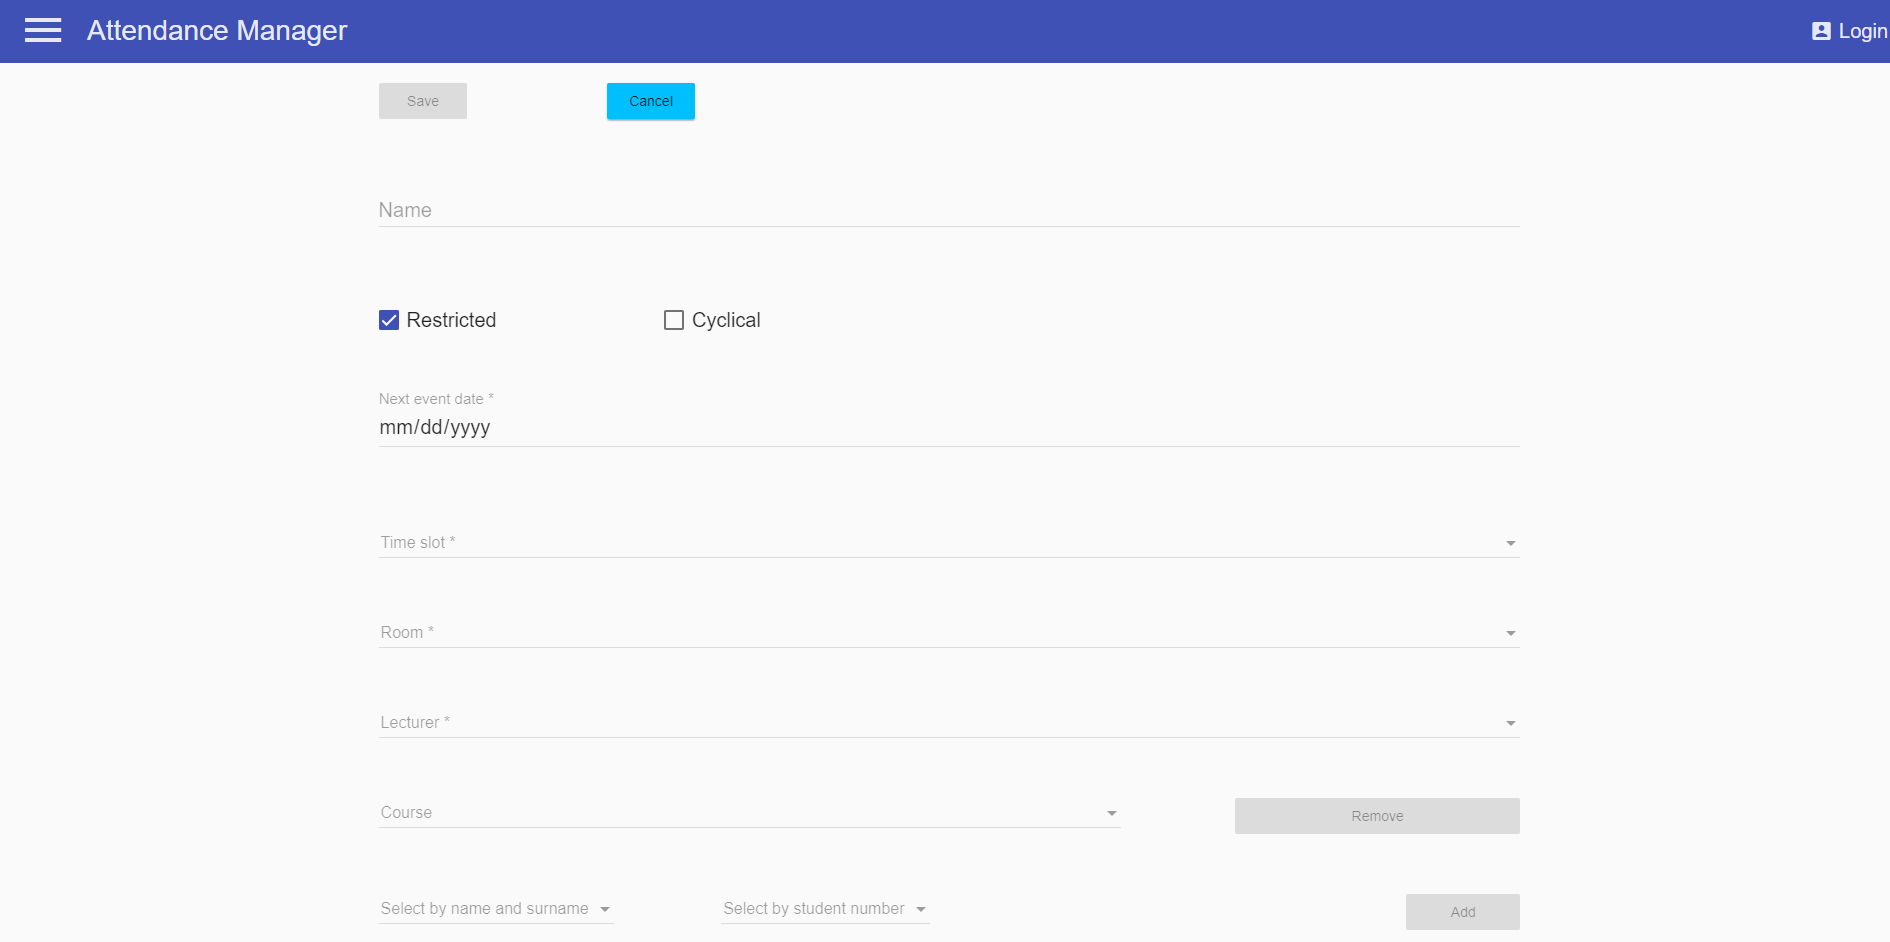
\includegraphics[height=8cm,width=15cm]{images/AddNewEvent}
Jest to strona służąca dodawaniu nowych wydarzeń. Zawiera ona formularz z odpowiednimi polami. Pola wymagane zostały odpowiednio oznaczone. Możliwość dodawania listy uczestników odblokowuje się po wybraniu opcji 'Restricted'.     % instrukcja użytkowania aplikacji
\newpage\section{Wdrożenie i testowanie systemu \NazwaSys} \label{sec:testy}
\subsection{Środowisko testowe}
% parametry komputera: procesor, liczba rdzeni, wielkość pamięci, karta graficzna, karta sieciowa, system operacyjny itp.
\subsection{Testy jednostkowe}
% https://pl.wikipedia.org/wiki/Test\_jednostkowy
\subsection{Analiza złożoności systemu \NazwaSys}
% tabele z czasami odpowiedzi 
% zajętości pamięci 
\subsection{Profilowanie kodu systemu \NazwaSys}
% analiza czasu wykonania programu 
\subsection{Wizualizacja działania systemu \NazwaSys}
% przedstawic graficznie struktury danych, dane i wyniki działania aplikacji 
% można wykorzystać SVG
\subsection{Ankieta}
% sformułować pytania ankietowe dla użytkowników systemu i osoby testującej
% przedstawić wyniki ankiety w postaci tabelarycznej i graficznej
% raportowanie błędów 
\subsection{Wnioski}
 
          % testy i dokumentacja użytkowa 
\newpage\section{Podsumowanie} \label{sec:podsumowanie}
 
   % podsumowanie i wnioski

% Literatura 
   \begin{thebibliography}{99}
    \addcontentsline{toc}{section}{Literatura}

	 \end{thebibliography}
 
     % literatura i źródłowe strony internetowe 
%Spis rysunków i tabel
\newpage\listoffigures
  \addcontentsline{toc}{section}{Spis rysunków}
\listoftables
  \addcontentsline{toc}{section}{Spis tabel}
 
          % Spis rysunkow i tabel
%\newpage\section{Dodatek} 
\newpage\section{Dodatki} 
%\newpage\textbf{Dodatki}\\
%\addcontentsline{toc}{section}{Dodatki}
\subsection{Instalacja systemu \NazwaSys}
\subsection{Instrukcja użytkownika systemu \NazwaSys}
\subsection{Instrukcja administratora systemu \NazwaSys}
\subsection{Treść ankiety systemu \NazwaSys}
 
        % Dodatek lub dodatki
\newpage\section{Załączniki}
\begin{itemize}
	\item treść pracy w formacie LATEX,
	\item implementację systemu \NazwaSys,
	\item kody uruchomieniowne systemu \NazwaSys. 
\end{itemize} 
      % Załącznik lub załączniki
\end{document}